\begin{singlespacing}
\chapter{The Standard Model and all that}
\label{chapter:theory}
%
\begin{epigraphs}
\qitem{%
The idea that theorems follow from the postulates does not correspond to simple
observation.
If the Pythagorean theorem were found to not follow from the postulates, we
would again search for a way to alter the postulates until it was true.
Euclid's postulates came from the Pythagorean theorem, not the other way.}%
{Richard~Hamming,
\textit{The Unreasonable Effectiveness of Mathematics},
1980~\cite{hamming1980unreasonable}}
\end{epigraphs}
\end{singlespacing}
\noindent
Standard Model of what? See Figure~\ref{fig:theory_slayer}.
\TODO{Write down the lagrangian.}
See Table~\ref{tab:theory_particles}.

\begin{figure}[tp]
\centering
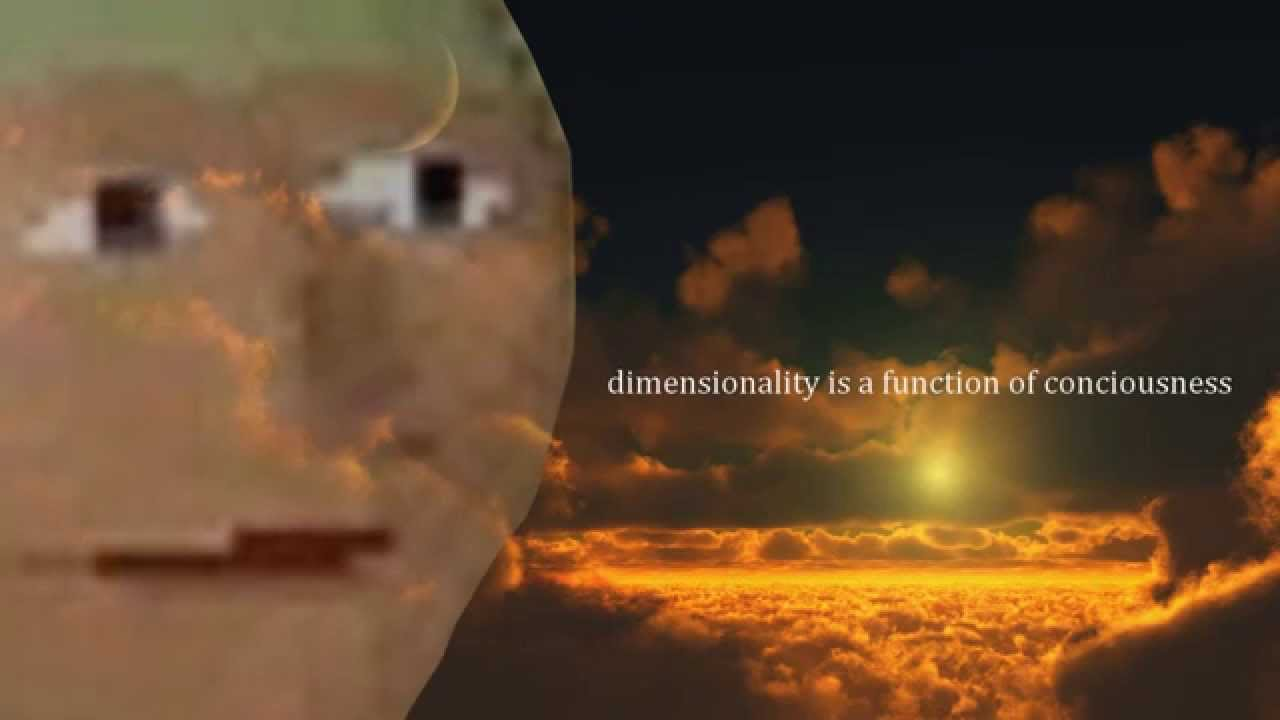
\includegraphics[width=0.618\textwidth]{figures/slayer.jpg}
\caption[
The short caption for your List of Figures
]{%
The short caption for your List of Figures should fit on one or two lines.
Longer captions go down here. I love slayer.%
}
\label{fig:theory_slayer}
\end{figure}

\begin{table}[tp]
\centering
\begin{tabular}{rrcccc}
fermions & quarks  & $j$ & $i$ & $h$ & Macarena\hphantom{!} \\
         &         & $g$ & $f$ & $e$ & Macarena\hphantom{!} \\[1ex]
         & laptons & $d$ & $c$ & $b$ & Macarena\hphantom{!} \\
         &         & $a$ & --- & --- & Macarena! \\
\end{tabular}
\caption[
Not particles of the Standard Model
]{%
Not particles of the Standard Model.
Sing along!%
}
\label{tab:theory_particles}
\end{table}

% this comment activates enlarged spacing for the final paragraph lol
